\section{Componentes em um diagrama}

Todo componente eletrônico possui uma \textbf{função}, ou seja, um \textbf{comportamento} que produz uma ação que atende a sua necessidade. Para que seu comportamento ocorra de modo esperado, todo componente possui \textbf{condições de operação}, sendo a principal dessas condições a alimentação.

A alimentação de um componente é a entrada de energia, que será processada e produzirá, através do comportamento do componente, uma nova forma de energia.

Utilizando a Figura \ref{fig:CircuitoDesafioComponentes} como exemplo, temos as seguintes conversões de energia:

\begin{minipage}{\linewidth}
  \centering
  \begin{minipage}{0.45\linewidth}
    Componentes:
    \begin{itemize}
      \item $V_{CC}$: \textbf{Fonte} - Converte energia química, no caso de pilhas ou baterias, em energia elétrica;
      \item $R_D$: \textbf{Resistor} - Converte energia elétrica em calor ao limitar a intensidade de corrente no seu ramo;
      \item $D$: \textbf{LED} - Converte energia elétrica em luz, permitindo que seja feita a sinalização luminosa, indicando que o circuito está ligado;
      \item $R_L$: \textbf{Resistor de carga} - Converte energia elétrica em calor, produzindo aquecimento do elemento.
    \end{itemize}
  \end{minipage}
  \hspace{0.05\linewidth}
  \begin{minipage}{0.45\linewidth}
    \begin{figure}[H]
      \centering
      \caption{Circuito elétrico}
      \label{fig:CircuitoDesafioComponentes}
      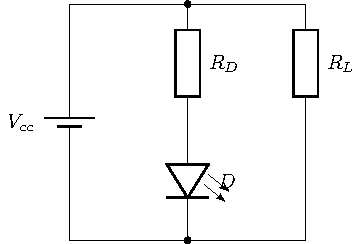
\includegraphics[scale=1.0]{fig-circuitoDesafio}
%
%      {\small Fonte: Próprio autor.}
    \end{figure}
  \end{minipage}
\end{minipage}


O circuito pode ser dividido em elemntos ativos e passivos, como mostrado na Figura \ref{fig:CircuitoDesafioFonteCarga}.

\begin{minipage}{\linewidth}
  \centering
  \begin{minipage}{0.45\linewidth}
    Assim temos:
    \begin{itemize}
      \item \textbf{Fonte}: A fonte é o \textbf{elemento ativo}, ou seja, é o que \textbf{fornece energia} ao restante dos componenentes deste circuito.
      \item \textbf{Carga}: São os \textbf{elementos passivos} do circuito, ou seja, aqueles que \textbf{consomem energia} da fonte.
    \end{itemize}
  \end{minipage}
  \hspace{0.05\linewidth}
  \begin{minipage}{0.45\linewidth}
    \begin{figure}[H]
      \centering
      \caption{Circuito elétrico}
      \label{fig:CircuitoDesafioFonteCarga}
      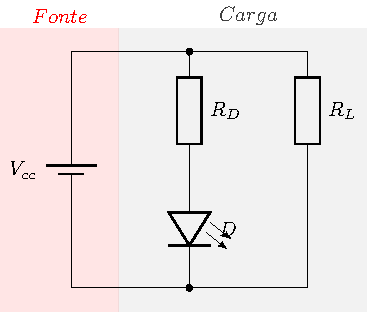
\includegraphics[scale=1.0]{fig-circuitoDesafioFonteCarga}
%
%      {\small Fonte: Próprio autor.}
    \end{figure}
  \end{minipage}
\end{minipage}
